\documentclass[10pt]{article}
\usepackage[french]{babel}
\usepackage[utf8]{inputenc}
\usepackage[T1]{fontenc}
\usepackage{amsmath}
\usepackage{amsfonts}
\usepackage{amssymb}
\usepackage[version=4]{mhchem}
\usepackage{stmaryrd}
\usepackage{graphicx}
\usepackage[export]{adjustbox}
\graphicspath{ {./images/} }

\begin{document}
\section*{Analyse Numérique - TD № 2-19-02-2025}
\section*{Exercice 1:}
On lance une fusée verticalement au sol et l'on mesure pendant les dernières 80 secondes l'accélération que l'on note \(v\) :

\begin{center}
\begin{tabular}{|c|c|c|c|c|c|c|c|c|c|}
\hline
\(\mathrm{t}(\mathrm{en} \mathrm{s})\) & 0 & 10 & 20 & 30 & 40 & 50 & 60 & 70 & 80 \\
\hline
\(\gamma\left(\mathrm{en} \mathrm{m} / \mathrm{s}^{2}\right)\) & 30 & 31,63 & 33,44 & 35,47 & 37,75 & 40,33 & 43,29 & 46,70 & 50,67 \\
\hline
\end{tabular}
\end{center}

Calculer la vitesse V de la fusée à l'instant \(\mathrm{t}=80 \mathrm{~s}\), par les trapèzes (formule composite) puis par Simpson (formule composite).

\section*{Exercice 2:}
Soit l'intégrale suivante :

\[
I=\int_{0}^{1} f(x) d x=\int_{0}^{1} 4 \sqrt{1-x^{2}} d x
\]

1- Montrer que \(I=\pi\) analytiquement en faisant le changement de variable \(\mathrm{x}=\cos (\mathrm{y})\);\\
2- Donner une approximation \(I_{1}\) du calcul de \(I\) en appliquant la méthode de Simpson sur 2 intervalles équirépartis entre 0 et 1 ;\\
3- Calculer le polynôme de Lagrange passant par 3 points \(\left(\mathrm{x}_{\mathrm{i}}, \mathrm{y}_{\mathrm{i}}\right):(0,4) ;(0.5,2 \sqrt{3}) ;(1,0)\) Calculer l'intégrale \(I_{2}\) du polynôme obtenu.

\section*{Exercice 3:}
Soit l'intégrale suivante : \(I=\int_{0}^{1} f(x) d x=\int_{0}^{1} x^{3} \exp (-x) d x\)\\
On se propose d'évaluer numériquement cette intégrale pour différentes quadratures :\\
\(\int_{a}^{b} f(x) d x \approx \sum_{j=0}^{n} w_{j} f\left(x_{j}\right)\)\\
où les \(x_{0}<x_{1}<\ldots<x_{n}\) sont les ( \(n+1\) ) nœuds et où \(w_{j}=\int_{a}^{b} L_{j}(x) d x\) avec \(L_{j}(x)\) le polynôme d'interpolation de Lagrange.

\section*{1- Calcul exact :}
En posant, \(I_{n}=\int_{0}^{b} x^{n} \exp (-x) d x\), montrer la relation de récurrence (on intégrera par parties) : \(I_{n}=-e^{-1}+n I_{n-1}\) Calculer la valeur exacte de l'intégrale \(I\).

2- Méthode des trapèzes :\\
Donner une approximation de cette intégrale en appliquant la méthode composite des trapèzes en utilisant 4 intervalles de longueur égale. La méthode des trapèzes sera appliquée sur chaque sous-intervalle.

\section*{3- Méthode de Simpson :}
Donner une approximation de cette intégrale en appliquant la méthode composite de Simpson en utilisant 2 intervalles de longueur égale. La méthode de Simpson sera appliquée sur chaque sous-intervalle.

4- Quadrature de Gauss :\\[0pt]
En effectuant un changement de variables, placez-vous dans l'intervalle [-1, 1]. Appliquer la quadrature de Gauss avec 3 points d'interpolation sur l'intervalle [-1, 1]. Ces points sont les racines du polynôme de Legendre de degré 3 qui vaut \(P_{3}(x)=\frac{1}{2}\left(5 x^{3}-3 x\right)\).

\begin{itemize}
  \item Calculer l'erreur relative et l'erreur absolue pour chaque méthode. Quelle est la moins coûteuse ? Quelle est la méthode la plus précise ?
\end{itemize}

\section*{Exercice 4:}
Un projectile est lancé avec une vitesse initiale \(\vec{V}_{0}\) à un angle de \(45^{\circ}\). Il est soumis uniquement à la pesanteur.

\begin{enumerate}
  \item En appliquant la relation fondamentale de la dynamique, montrer qu'on obtient un système de deux équations différentielles de deuxième ordre à résoudre :
\end{enumerate}

\[
\left\{\begin{array}{c}
\frac{d^{2} x}{d t^{2}}=0 \\
\frac{d^{2} y}{d t^{2}}=-g
\end{array}\right.
\]

\begin{enumerate}
  \setcounter{enumi}{1}
  \item Ecrire le système d'équations différentielles sous forme d'un problème de Cauchy.
  \item Déterminer sa vitesse et sa position au cours du temps grâce à la méthode d'Euler explicite. On exprimera pour cela le terme général des suites \(\left(\mathrm{x}_{\mathrm{n}}\right),\left(\mathrm{y}_{\mathrm{n}}\right),\left(\mathrm{v}_{\mathrm{n}}\right)\) et \(\left(\mathrm{u}_{\mathrm{n}}\right)\) correspondant aux composantes suivant x et y des vecteurs position et de vitesses respectivement.
  \item Calculer les valeurs des positions et vitesses pour 3 itérations avec :
\end{enumerate}

Les vitesses à l'instant initial \(\mathrm{v}_{0}\) et \(\mathrm{u}_{0}\) sont égales à \(1 \mathrm{~m} / \mathrm{s}\), le pas d'intégration h est égale \(10^{-4} \mathrm{~s}\)\\
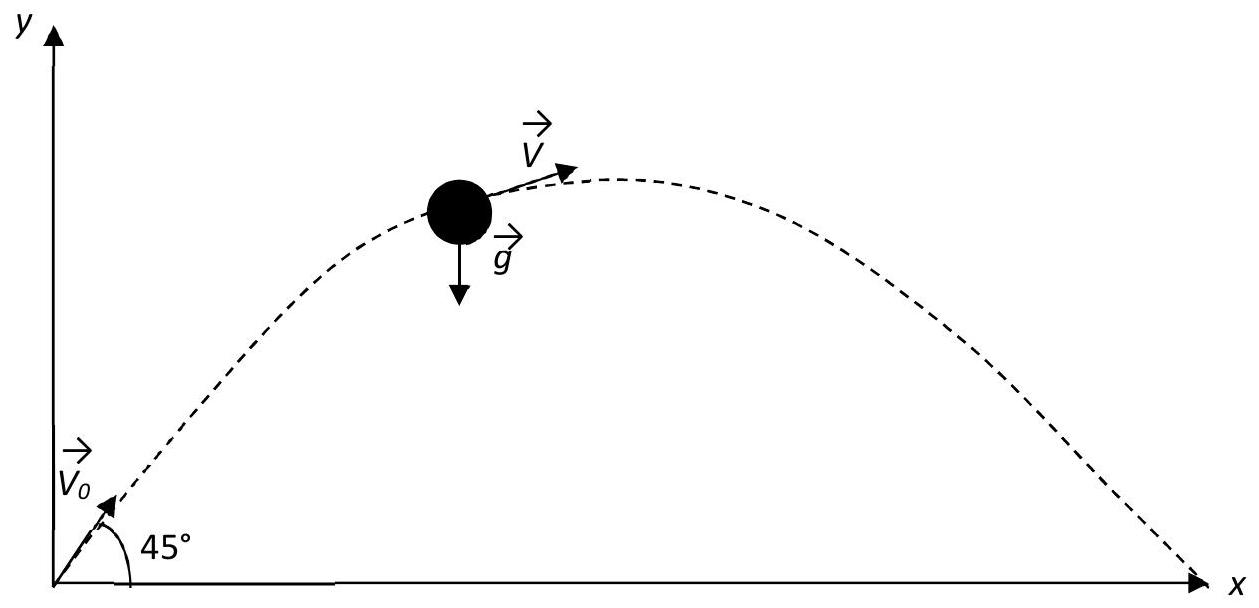
\includegraphics[max width=\textwidth, alt={}, center]{13684ccf-0e12-4e73-b2f2-c800b5dfa129-2_608_1259_1615_322}

\section*{Exercice 5:}
Soit l'équation différentielle ordinaire (EDO) suivante :

\[
y^{\prime}(t)=f(t, y(t))=1+t^{2}+y(t)
\]

avec la condition initiale \(\mathrm{y}_{0}=\mathrm{y}(\mathrm{t}=0)=1\).

\begin{enumerate}
  \item Ecrire l'équation discrète en utilisant le schéma d'Euler explicite;
  \item En utilisant le pas de temps \(h=0.1\) calculer \(y_{1}=y(0.1)\) et \(y_{2}=y(0.2)\) (donner les résultats en arrondissant et en gardant au moins 3 décimales) ;
  \item On souhaite améliorer la prédiction du schéma numérique en utilisant la méthode d'Euler améliorée (prédicteur-correcteur) suivante :
\end{enumerate}

\[
\left\{\begin{array}{c}
\tilde{y}_{n+1}=y_{n}+h f\left(t_{n}, y_{n}\right) \\
y_{n+1}=y_{n}+h f\left(t_{n+1}, \tilde{y}_{n+1}\right)
\end{array}\right.
\]

Ecrire l'équation discrète correspondant à cette méthode ;\\
4. Calculer de nouveau \(y_{1}=y(0.1)\) et \(y_{2}=y(0.2)\) toujours avec un pas de temps \(h=0.1\) (donner les résultats en arrondissant et en gardant au moins 3 décimales).


\end{document}